% !BIB TS-program = biber

% -*- coding: utf-8 -*-
\documentclass{scrbook}[headings=normal]% Entspricht den Typografieregeln eines Buches
\usepackage{wbh-thesis} % Laden der Vorlage
\usepackage{blindtext}
\usepackage{listings}
\usepackage[automark,headsepline]{scrlayer-scrpage}
\renewcommand{\lstlistingname}{Quelltext}% Listing -> Quelltext
\renewcommand{\lstlistlistingname}{Quellcodeverzeichnis}

\KOMAoptions{%
    headsepline=true,   % header line
    footsepline=false,          % footer line
    plainheadsepline=false, % activate header line for plain pages
    plainfootsepline=false} % activate footer line for plain pages

\usepackage{mathtools}

\usepackage[framemethod=tikz]{mdframed}

% Shorthands
\newcommand*\iffdef{\overset{\text{def}}{\iff}}
\DeclarePairedDelimiter\abs{\lvert}{\rvert}
\DeclarePairedDelimiter\norm{\lVert}{\rVert}

\definecolor{WBH}{RGB}{0, 94, 166}

% Theorem
\mdtheorem[
  linecolor=WBH,
  frametitlefont=\sffamily\bfseries\color{white},
  frametitlebackgroundcolor=WBH,
]{Def}{Defintion}


\definecolor{codegreen}{rgb}{0,0.6,0}
\definecolor{codegray}{rgb}{0.5,0.5,0.5}
\definecolor{codepurple}{rgb}{0.58,0,0.82}
\definecolor{backcolour}{rgb}{0.95,0.95,0.92}

\definecolor{maroon}{rgb}{0.5,0,0}
\definecolor{darkgreen}{rgb}{0,0.5,0}

\lstdefinestyle{Codestyle}{
    backgroundcolor=\color{backcolour},   
    commentstyle=\color{codegreen},
    keywordstyle=\color{magenta},
    numberstyle=\tiny\color{codegray},
    stringstyle=\color{codepurple},
    basicstyle=\ttfamily\footnotesize,
    breakatwhitespace=false,         
    breaklines=false,                 
    captionpos=b,                    
    keepspaces=false,     
    columns=fullflexible,            
    numbers=left,                    
    numbersep=5pt,                  
    showspaces=false,                
    showstringspaces=false,
    showtabs=false,                  
    tabsize=1
}

\lstdefinelanguage{XML}
{
  morestring=[b]",
  moredelim=[s][\bfseries\color{maroon}]{<}{\ },
  moredelim=[s][\bfseries\color{maroon}]{</}{>},
  moredelim=[l][\bfseries\color{maroon}]{/>},
  moredelim=[l][\bfseries\color{maroon}]{>},
  morecomment=[s]{<?}{?>},
  morecomment=[s]{<!--}{-->},
  commentstyle=\color{darkgreen},
  stringstyle=\color{blue},
  identifierstyle=\color{red}
}

\lstset{style=Codestyle}


\pagestyle{scrheadings}
\clearscrheadfoot

\ihead{\leftmark}
\ohead{\pagemark} 


  \begin{document}
  \begin{titlepage}
\begin{center}
\newcommand{\HRule}{\rule{.9\linewidth}{.6pt}} % New command to make the lines in the title page

\vspace*{.06\textheight}
{\scshape\LARGE Wilhelm Büchner Hochschule}\vspace{1.5cm} % University name
\textsc{\Large Masterthesis}\\[0.5cm] % Thesis type

\HRule \\[0.4cm] % Horizontal line


\Large\textbf{ Realisierung eines Source-to-Source Compilers zwischen Xamarin.Forms und Flutter zur automatisierten Transformation bestehender mobiler 
Anwendungen}\par


\HRule \\[1.5cm] % Horizontal line
 
\begin{minipage}[t]{0.4\textwidth}
\begin{flushleft} \large
\emph{Author:}\\
Julian Pasqué % Author name - remove the \href bracket to remove the link
\end{flushleft}
\end{minipage}
\begin{minipage}[t]{0.4\textwidth}
\begin{flushright} \large
\emph{Betreuer:} \\
Dr. Thomas Kalbe % Supervisor name - remove the \href bracket to remove the link  
\end{flushright}
\end{minipage}\\[3cm]
 
\vfill


\large Verteilte und mobile Anwendungen\\[0.8cm] % Research group name and department name
\large Fachbereich Informatik\\[0.8cm] % Research group name and department name
\large Matrikelnummer: 902953 \\[0.8cm] % Research group name and department name
 
\vfill

{\large \today}\\[6cm] % Date
 
\vfill
\end{center}
\end{titlepage}  % Setzt die Titelseite
  \frontmatter        % Eigenschaften für den Vorspann setzen
  
  \include{Abstract}  % Setzt die Titelseite

  \tableofcontents    % Setzt das Inhaltsverzeichnis
  \listoffigures      % Setzt das Abbildungsverzeichnis
  
  \listoftables       % Setzt das Tabellenverzeichnis
  
  \lstlistoflistings

  \mainmatter         % Eigenschaften für den Hauptteil setzen
  
  \chapter{Einleitung}
Die Entwicklung von verschiedenen mobilen Geräten mit unterschiedlichsten Hardwarekomponenten und Betriebssystemen hat einen stark fragmentierten Markt ergeben.\footcite[Vgl.][S. 3]{Joorabchi2016}  Diese Situation hat einen direkten Einfluss auf die Softwareentwicklung, da die dedizierte Programmierung für die einzelnen Plattformen ressourcenintensiv ist.  Durch Realisierung von Web- und hybriden Apps können Softwareprojekte von der darunterliegenden Plattform abstrahieren und plattformübergreifend verwendet werden.  Diese Anwendungen haben jedoch, wie schon ausführlich im wissenschaftlichen Diskurs ausgeführt,  eine schlechtere Performance und nur begrenzt Zugriff auf die plattformspezifischen Funktionalitäten.  \footcite[Vgl.][S. 110ff.]{Barton2016} 

Durch die Kombination der Vorteile von Web- und hybriden Anwendungen mit denen von nativen konnten Frameworks wie Xamarin.Forms und Flutter Programmierern die Möglichkeit bieten,  ihre Anwendungen auf mehreren Plattformen bereit zu stellen.  Diese Apps haben neben einer guten Performance auch Zugriff auf sämtliche plattformspezifischen Funktionalitäten.  Durch die Abstraktion von Hardware und Betriebssystem können Apps mit einer gemeinsamen Quelltextbasis und somit mit geringerem Ressourcenaufwand entwickelt werden. \footcite[Vgl.][S. 295]{Vollmer2017} 

Der Möglichkeit, Ressourcen zu sparen, steht das Risiko der Abhängigkeit gegenüber, da sich die oben genannten Frameworks zur Cross-Plattform-Entwicklung in den verwendeten Programmiersprachen sowie ihrer Arbeitsweise grundlegend unterscheiden.  Ein Wechsel zwischen den einzelnen Alternativen ist daher mit enormen Arbeitsaufwänden verbunden. \footcite[Vgl.][S. 64]{Wissel2017}  

\section{Motivation}
Im Mai 2020 hat Microsoft mit dem .NET \ac{maui} einen Nachfolger für das Xamarin.Forms Framework angekündigt, der im Herbst 2021 zusammen mit der sechsten Hauptversion des .NET Frameworks veröffentlicht werden soll. Zum aktuellen Zeitpunkt ist bereits bekannt, dass der Umstieg grundlegende Änderungen mit sich bringt und Anwendungen,  die mit Hilfe von Xamarin.Forms entwickelt wurden,  angepasst werden müssen.\footcite[Vgl.][Abgerufen am 28.10.2020]{Hunter2020}

Für Xamarin.Forms Entwickler wird es also unausweichlich sein,  tiefgreifende Modifizierungen an bereits realisierten Anwendungen vorzunehmen,  um in der Zukunft von Aktualisierungen zu profitieren.  Unternehmen und einzelne Programmierer stehen vor der Entscheidung,  ob ein Umstieg auf das leistungsfähige Flutter sinnvoller ist,  als die Anpassungen für das neue noch nicht erprobte .NET \ac{maui},  das federführend von einer Firma entwickelt wird,  welche leichtfertig mit der Abhängigkeit von Entwicklern umgeht.

Ein automatisierter Umstieg auf das von Google entwickelte Framework Flutter würde also nicht nur die Anpassungen an .NET \ac{maui} vermeiden,  sondern die mobile Anwendung auf eine vermeintlich zukunftssichere Basis stellen.  Denn obwohl Google in der Vergangenheit schon manche Projekte eingestellt hat,  wie zum Beispiel Google Nexus oder Google Hangouts,  ist damit bei Flutter aufgrund des Erfolges nicht zu rechnen.  Nach offizieller Aussage von Tim Sneath, dem Produkt Manager des Frameworks,  haben im Jahr 2020 mehr als zwei Milliotatanen Entwickler Flutter verwendet und über 50.000 mobile Anwendungen programmiert. \footcite[Vgl.][Abgerufen am 28.10.2020]{Sneath2020} Neben der hohen Verbreitung des Frameworks,  konnte das Portal Stackoverflow in seinen jährlichen Umfragen auch eine hohe Beliebtheit unter Softwareentwicklern in den Jahren 2019\footcite[Vgl.][Abgerufen am 28.10.2020]{Stack2019} und 2020\footcite[Vgl.][Abgerufen am 28.10.2020]{Stack2020} ermitteln.  Im März 2021 hat Google darüber hinaus die zweite Hauptversion von Flutter veröffentlicht,  welche zusätzlich Support für die Entwicklung von Webseiten zur Verfügung stellt. \footcite[Vgl.][Abgerufen am 28.10.2020]{GoogleFlutter2}


\section{Ziel der Arbeit}
Im Rahmen dieser Arbeit soll ein Source-To-Source Compiler zwischen den Frameworks Xamarin.Forms und Flutter realisiert werden, mit dessen Hilfe die folgende zentrale Forschungsfrage beantwortet werden soll: "Können Apps komplett automatisiert von Xamarin.Forms zu Flutter übersetzt werden, oder sind manuelle Arbeitsschritte erforderlich?"

\section{Gliederung}
Um diese Forschunsgfrage beantworten zu können, wird in Kapitel \ref{chap:Compiler} auf die theoretischen Grundlagen von Software-Übersetzern eingegangen.  Anschließend wird in Kapitel \ref{chap:CompilerEntwurf} auf den Entwurf des in dieser Arbeit zu implementierenden Compiler eingegangen, bevor in Kapitel \ref{chap:CrossPlattformFrameworks} die Unterschiede zwischen den Frameworks Xamarin.Forms und Flutter behandelt werden.  Die Unterschiede zwischen den Programmiersprachen werden in Kapitel \ref{chap:Programmiersprachen} behandelt. Darauf aufbauend wird in Kapitel \ref{chap:Realisierung} der Source-To-Source Compiler realisiert und in dem darauf folgen Kapitel \ref{chap:Qualitätssicherung} getestet bevor in Kapitel \ref{chap:FazitAusblick} die Forschungsfrage beantwortet und ein Fazit gezogen wird. 
  \chapter{Compiler}
\label{chap:Compiler}

Programmiersprachen dienen als Verständigungsmittel zwischen Programmierern und Rechenanlagen wie z.B Smartphones.  Diese Sprachen haben sich in der Vergangenheit dabei immer mehr an die  Terminologie eines bestimmtes Anwendungsgebietes angenähert. Durch diese Entwicklung eigneten sich Programmiersprachen direkt für die Dokumentation von entwickelten Algorithmen und Anwendungen, entfernten sich jedoch weiter von den Gegebenheiten des realen Rechners.\footcite[Vgl.][S. 15]{Schneider1975} Die Beziehung zwischen Softwareentwicklern und Rechenanlagen mit Hilfe von Programmiersprachen werden in Abbildung \ref{fig:Programmiersprachen als Schnittstelle} dargestellt. 

\begin{figure}[!ht]
 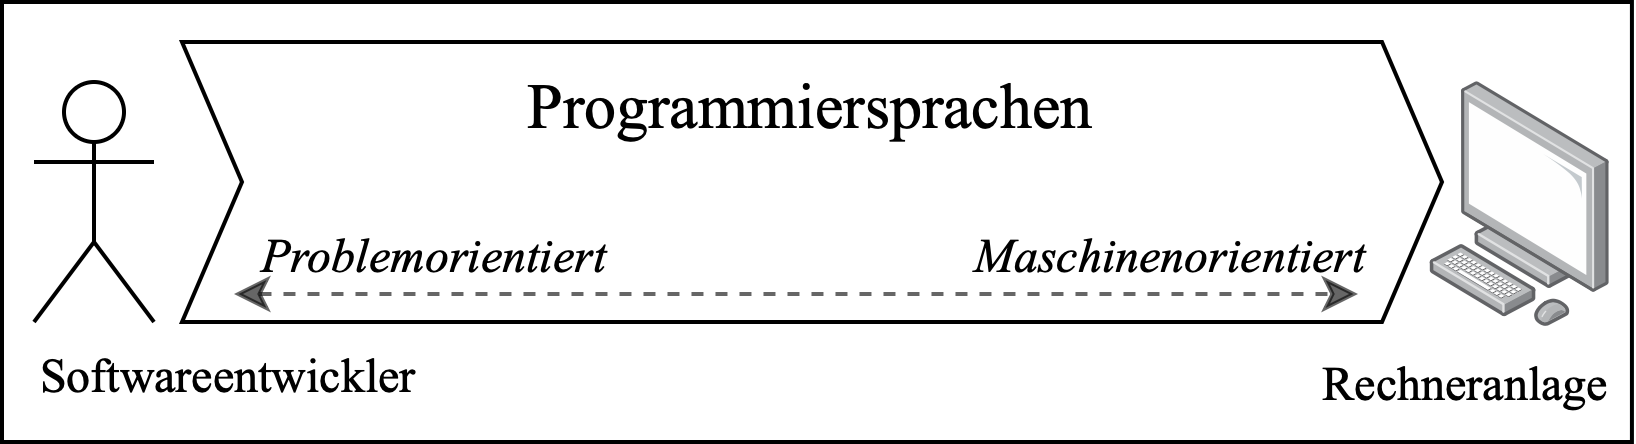
\includegraphics[width=\textwidth,height=\textheight,keepaspectratio]{Images/LanguageIntermediary.png}
 \caption{Programmiersprachen als Schnittstelle}
 \label{fig:Programmiersprachen als Schnittstelle}
\end{figure}

Für die Ausführung einer in einer problemorientierten Programmiersprache geschriebenen Anwendung ist es notwendig, die Sprache in eine maschinenorientierte Form zu überführen. \footcite[Vgl.][S. 15]{Schneider1975} Bereits im Jahre 1952 stelle Rutishauser fest,  dass Computer in der Lage sind,  diesen Übersetzungsvorgang selbst durchzuführen.\footcite[Vgl.][S. 312]{Rutishauser1952} 
Durch die Möglichkeit zur automatischen Übersetzung von problemorientierten Programmiersprachen konnten Hochsprachen entwickelt werden, die menschenfreundliche Sprachelemente anstatt Maschineninstruktionen verwenden. \footcite[Vgl.][S. 47]{Wagenknecht2014}
\section{ Grundbegriffe}
Diese historische Einführung zeigt,  dass Software zur automatisierten Übersetzung schon seit der Mitte des letzten Jahrhunderts thematisiert wurde, so hat sich in der Wissenschaft eine einheitliche Definition ergeben.  \citeauthor{Ullmann2008} beschreibt die sogenannten Compiler im Jahre \citeyear{Ullmann2008} wie folgt:\footcite[Vgl.][S. 1]{Ullmann2008} 
\begin{Def}[Compiler]
Ein Compiler ist ein Programm, welches ein anderes Programm aus einer Quellsprache in ein gleichwertiges Programm einer Zielsprache übersetzen kann.
\end{Def} 
\vspace{-1em}

Aus dieser Definition lässt sich ein für diese Arbeit relevanter Fakt ableiten: Compiler sind nicht ausschließlich Übersetzer  zwischen problemorientierten und maschinenorientierten Programmiersprachen.  Sie sind ausschließlich für die Übersetzung von einer Quellsprache in eine Zielsprache verantwortlich.  Auch wenn der Begriff Programm für jedermann geläufig ist,  kann es  passieren,  dass von verschiedenen Repräsentationen gesprochen wird.  So können alle drei der folgenden Begriffe als Programm bezeichnet werden: Der Quelltext,  das ausführbare Programm und der laufende Prozess auf einem Computer.  Für das weitere Verständnis dieser Arbeit ist mit dem Begriff Programm die ausführbare Anwendung auf den Smartphones des Anwenders gemeint.  

Neben der Übersetzung von problem- zu maschinenorientierter Sprache gibt es ebenfalls Compiler, die andere Ziele verfolgen. Dazu gehören zum Beispiel die sogenannten Binärübersetzer,  die den Binärcode eines Programmes für andere Rechner übersetzen, sodass er auf diesen ausgeführt werden kann.  \footcite[Vgl.][S. 27]{Ullmann2008} Ein
\ac{s2s} Compiler,  häufig auch als \glqq Transpiler\grqq{} bezeichnet,  ist ebenfalls eine besondere Ausprägung eines Compilers, die sich wie folgt definieren lässt.  \footcite[Vgl.][S. 1629]{IJCSIT2015}
\begin{Def}[Source-to-Source Compiler]
Ein Source-to-Source-Compiler ist ein Compiler, bei dem sowohl die Quellsprache als auch die Zielsprache eine Hochsprache ist.
\end{Def}
\vspace{-1em}

Der Begriff Hochsprache ist dabei ein Synonym für die bereits eingeführten problemnahen Sprachen wie zum Beispiel C++,  Java,  \Csharp  oder Dart und damit für den Menschen in einer lesbaren und änderbaren Form geschrieben sind. \footcite[Vgl.][S. 9]{Eisenecker2008} 

\section{Compiler Struktur}
Zur Übersetzung von Programmen bearbeiten Compiler zwei Teilaufgaben,  die Analyse und die Synthese. Während der Analyse wird das Programm in seine Bestandteile zerlegt und mit einer grammatikalischen Struktur versehen. Diese wird anschließend verwendet, um eine Zwischendarstellung zu generieren.  Dabei wird überprüft, ob das Programm syntaktisch und semantisch fehlerfrei ist oder ob der Programmierer Änderungen vornehmen muss. \footcite[Vgl.][S. 6f]{Ullmann2008} Der Begriff Syntax beschreibt den Aufbau eines Programmes,  sie legt fest wie Sprachelemente aus anderen Sprachelementen zusammengesetzt sind.  Im Gegensatz dazu beschreibt die Semantik die Bedeutung der Programmen und regelt die Bedeutung von Sprachelementen.  \footcite[Vgl.][S. 36]{Schneider1975}  Außerdem werden bei der Analyse Informationen über das Quellprogramm gesammelt und in der so genannten Symboltabelle abgelegt.  Die Synthese konstruiert aus der Zwischendarstellung und den Informationen aus der Symboltabelle das gewünschte Zielprogramm.  Der Teil des Compilers, der sich mit der Analyse befasst wird oft als Front-End bezeichnet, derjenige der für die Synthese zuständig ist als Back-End.  \footcite[Vgl.][S. 6f]{Ullmann2008}

Der Vorgang des Kompilierens lässt sich basierend auf diesen zwei Teilaufgaben nach \citeauthor{Ullmann2008} in mehrere Phasen unterteilen,  die in Abbildung \ref{fig:Compilerphasen} grafisch dargestellt sind und in diesem Abschnitt detailliert beschrieben werden.  \footcite[Vgl.][S. 6]{Ullmann2008}

\begin{figure}[!ht]
 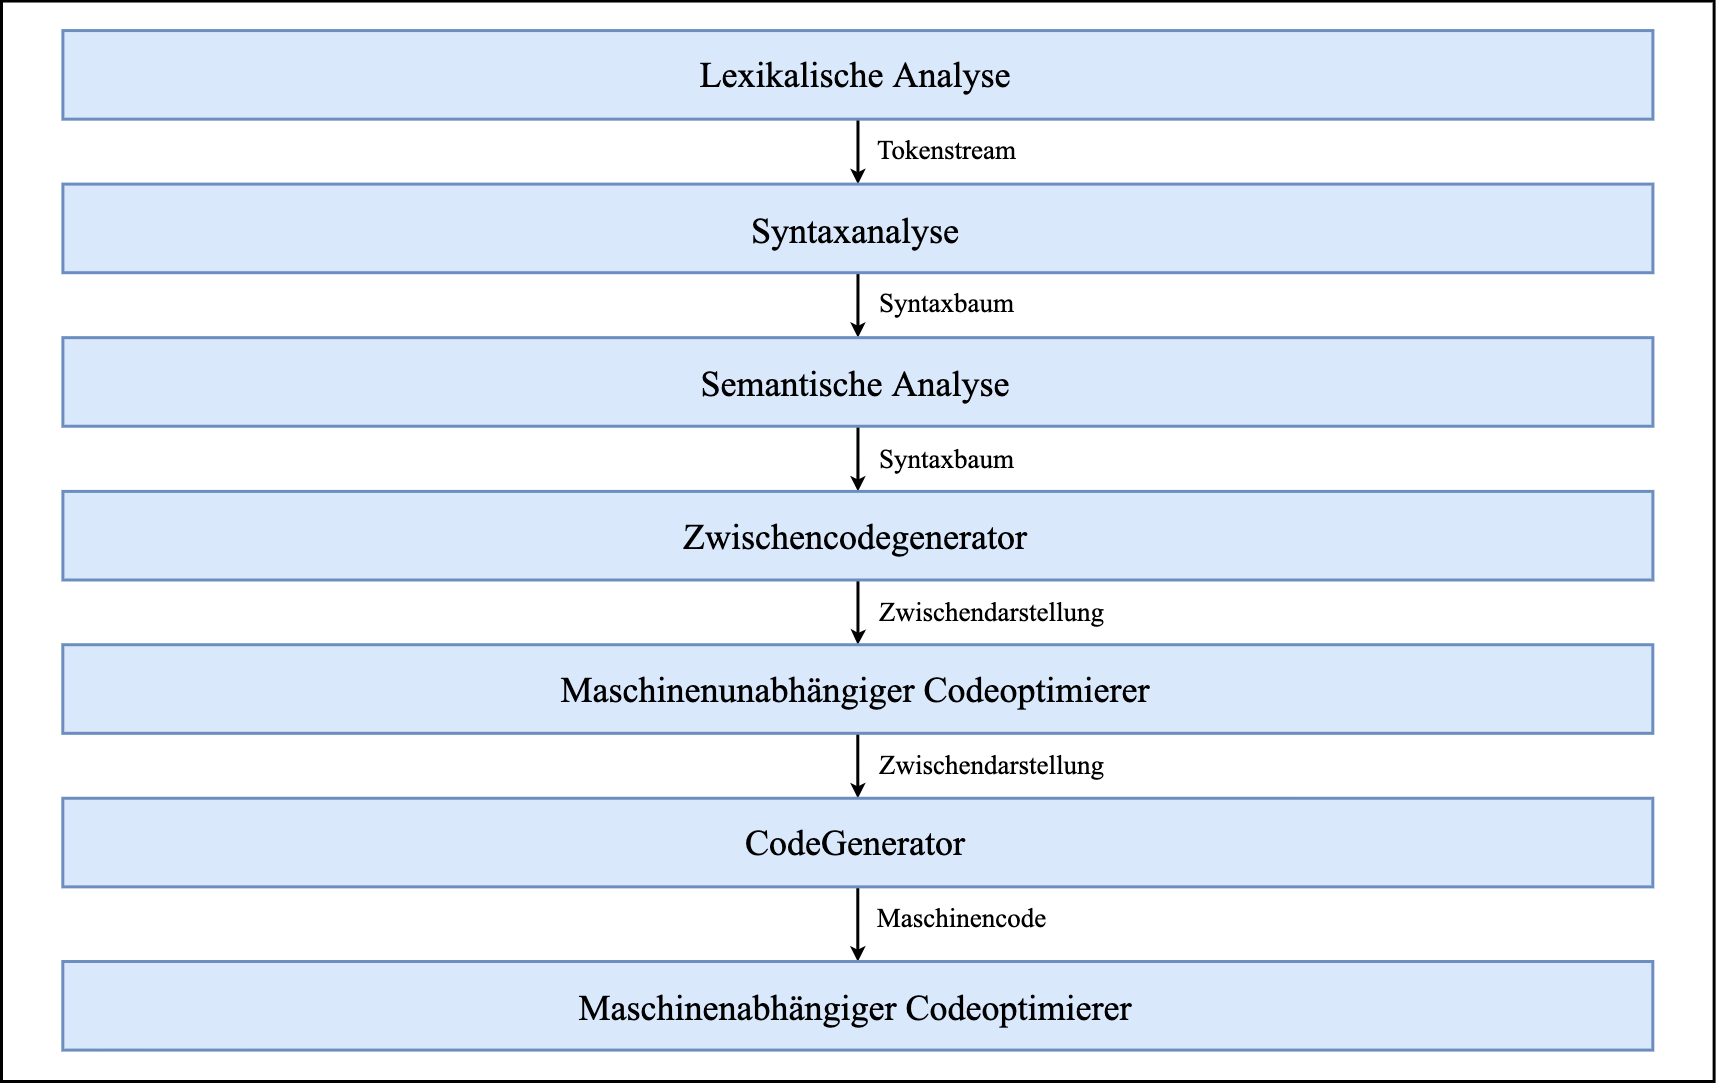
\includegraphics[width=\textwidth,keepaspectratio]{Images/Compiler/Phasen.png}
 \caption[Phasen eines Compilers]{Phasen eines Compilers\protect\footcite{Ullmann2008}}
 \label{fig:Compilerphasen}
\end{figure}
\footnotetext{Abbildung in Anlehnung an Ullman et al. 2008, S.6.}


\section{Lexikalische Analyse}
Die erste Phase eines Compilers ist die lexikalische Analyse,  die den Quelltext in Lexeme untergliedert.  Ein Lexem ist die Folge von Zeichen im Quellprogramm,  die als Instanz eines Tokens erkannt wurden.  Dabei ist ein Token ein Paar aus Namen und einem optionalen Attributwert,  wobei der Name zum Beispiel ein bestimmtes Schlüsselwort, oder eine Folge von Eingabezeichen sein kann und der Attributwert auf einen Eintrag in der Symboltabelle verweist.  \footcite[Vgl.][S. 135 f.]{Ullmann2008} In Tabelle \ref{tab:Tokens} werden einige beispielhafte Tokens aufgeführt sowie die Information darüber, aus welchen Lexemen diese extrahiert werden.

\begin{table}[!ht]
\begin{tabularx}{\textwidth}{l|X|l}
   \textbf{Token} & \textbf{Beschreibung} & \textbf{Lexem} \\
\hline
if             & Zeichen i,f           & if                      \\ 
comparison     & Vergleichsoperatoren  & \textless{}=            \\ 
id             & Buchstaben            & pi                      \\ 
number         & Numerische Konstanten    & 3.14159                  
\end{tabularx}
\caption[Token-Beispiele]{Token-Beispiele \protect\footcite{Ullmann2008}}
 \label{tab:Tokens}
\end{table}
\footnotetext{Vgl. Ullman et al.  2008, S. 137.}

Der Teil eines Compilers,  der die Lexikalische Analyse durchführt,  wird als Lexer bezeichnet.  Basierend auf der beschriebenen Arbeitsweise ist in \ref{fig:LexerResult} ein Beispiel dargestellt, das zeigt wie der Lexer aus einer Zeichenfolge mehrere Tokens mit den optionalen Attributwerten extrahiert.  
 
\begin{figure}[!ht]
 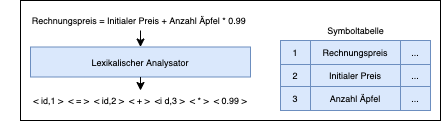
\includegraphics[width=\textwidth,keepaspectratio]{Images/Compiler/LexerResult.png}
 \caption[Lexer Beispiel]{Lexer Beispiel\protect\footcite{Ullmann2008}}
 \label{fig:LexerResult}
\end{figure}
\footnotetext{Abbildung in Anlehnung an Ullman et al. 2008, S.10.}

Der Lexer interagiert mit anderen Komponenten eines Compilers,  dies wird in Abbildung \ref{fig:LexerInteraktionen} visualisiert.  Klassischerweise wird der Lexer über den sogenannten Parser, welcher im nächsten Abschnitt eingeführt wird,  zur Übermittlung von Tokens aufgefordert,  dies wird in der Abbildung mit dem Aufruf "getNextToken" dargestellt.  \footcite[Vgl.][S. 135]{Ullmann2008} 

\begin{figure}[!ht]
 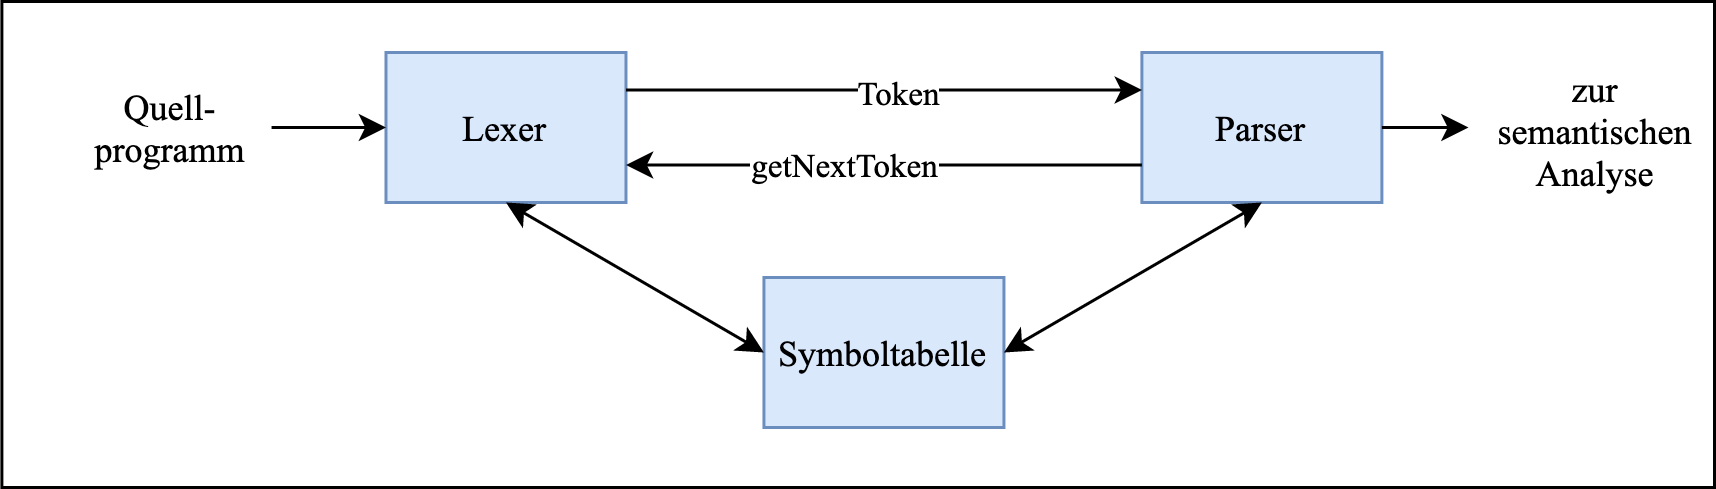
\includegraphics[width=\textwidth,keepaspectratio]{Images/Compiler/LexerParser.png}
 \caption[Interaktion zwischen Lexer und Parser]{Interaktion zwischen Lexer und Parser\protect\footcite{Ullmann2008}}
 \label{fig:LexerInteraktionen}
\end{figure}

Da der Lexer derjenige Teil des Compilers ist, der den Quelltext liest, kann er neben der Identifikation von Lexemen auch weitere Aufgaben übernehmen. So eignet er sich ideal zum Streichen von Kommentaren im Quelltext und zum Entfernen von Leerstellen,  wie Leerzeichen und Tabulatoren.  Zudem kann er gefundene Fehler den entsprechenden Zeilennummern zuordnen und dem Entwickler während der Kompilierung so einen genauen Hinweis auf den Ort des Fehlers geben. \footnotetext{Abbildung in Anlehnung an Ullman et al. 2008, S.135.} \footcite[Vgl.][S. 135.]{Ullmann2008} 
Häufig werden Lexer daher in zwei kaskadierende Prozesse unterteilt, einen für das Löschen von Kommentaren und Zusammenfassung von Leerraumzeichen und einen für die eigentliche lexikalische Analyse.  \footcite[Vgl.][S. 136.]{Ullmann2008} 

\section{Syntaxanalyse}
In der zweiten Phase, der Übersetzung, der Syntaxanalyse,  werden durch den bereits erwähnten Parser auch syntaktischer Analysator genannt,  die vom Lexer ausgegebenen Tokens in eine baumartige Zwischendarstellung überführt, die die grammatikalische Struktur der Tokens zeigt.  Diese Darstellung wird basierend auf ihrem Aussehen häufig als Syntaxbaum bezeichnet.  Die Knoten im Syntaxbaum stehen für eine Operation und die Kindknoten für die Argumente dieser Operation.  Die Anordnung der Operationen stimmt mit üblichen arithmentischen Konventionen überein,  wie zum Beispiel dem Vorrang der Multiplikation vor Addition. \footcite[Vgl.][S. 9]{Ullmann2008} Abbildung \ref{fig:ParserResult} zeigt die Erstellung eines Syntaxbaumes aus den Tokens  der Abbildung \ref{fig:LexerResult}.  Anhand des Knotens <id, 1> ist jederzeit über die Symboltabelle bekannt,  dass das Ergebnis der Rechnung an den Speicherort des Bezeichners Rechnungspreis abgelegt werden muss. \footcite[Vgl.][S. 9.]{Ullmann2008} 

\begin{figure}[!ht]
 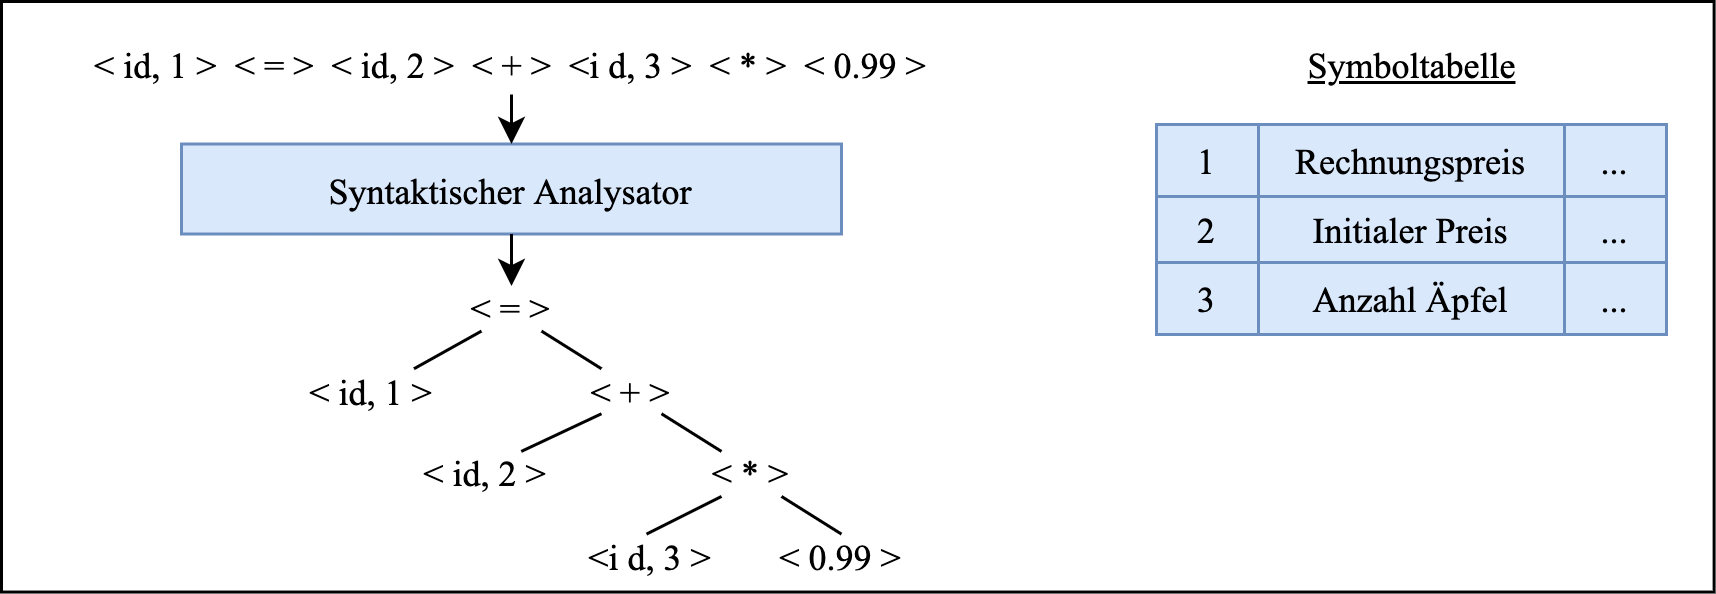
\includegraphics[width=\textwidth,keepaspectratio]{Images/Compiler/ParserResult.png}
 \caption[Syntaxbaum]{Syntaxbaum \protect\footcite{Ullmann2008} }
 \label{fig:ParserResult}
\end{figure}
\section{Semantische Analyse}

Bei der semantischen Analyse wird der Syntaxbaum  \footnotetext{Abbildung in Anlehnung an Ullman et al. 2008, S.10.}  als Aufgliederung der Programmkonstruktur,  zusammen mit den Informationen aus der Symboltabelle verwendet,  um das Quellprogramm auf semantische Konsistenz mit der Sprachdefinition zu überprüfen. \footcite[Vgl.][S. 157]{Wilhelm2012}.  Zudem werden hier Typinformationen gesammelt und zur späteren Verwendung im Syntaxbaum oder der Symboltabelle hinterlegt.  Auch findet eine Typüberprüfung statt die analysiert, ob jeder Operator die passenden Operanden hat.  So wird beispielsweise validiert,  ob ein Index eine Ganzzahl ist.  Es besteht die Möglichkeit, innerhalb des Baums Typkonvertierungen zu deponieren.  So wurde in dem bisherigen Beispiel die Anzahl Äpfel als Ganzzahl behandelt und wird für die Berechnung des Preises in Abbildung \ref{fig:Typ} zu einer Fließkommazahl konvertiert. \footcite[Vgl.][S. 9ff]{Ullmann2008}

\begin{figure}[!ht]
 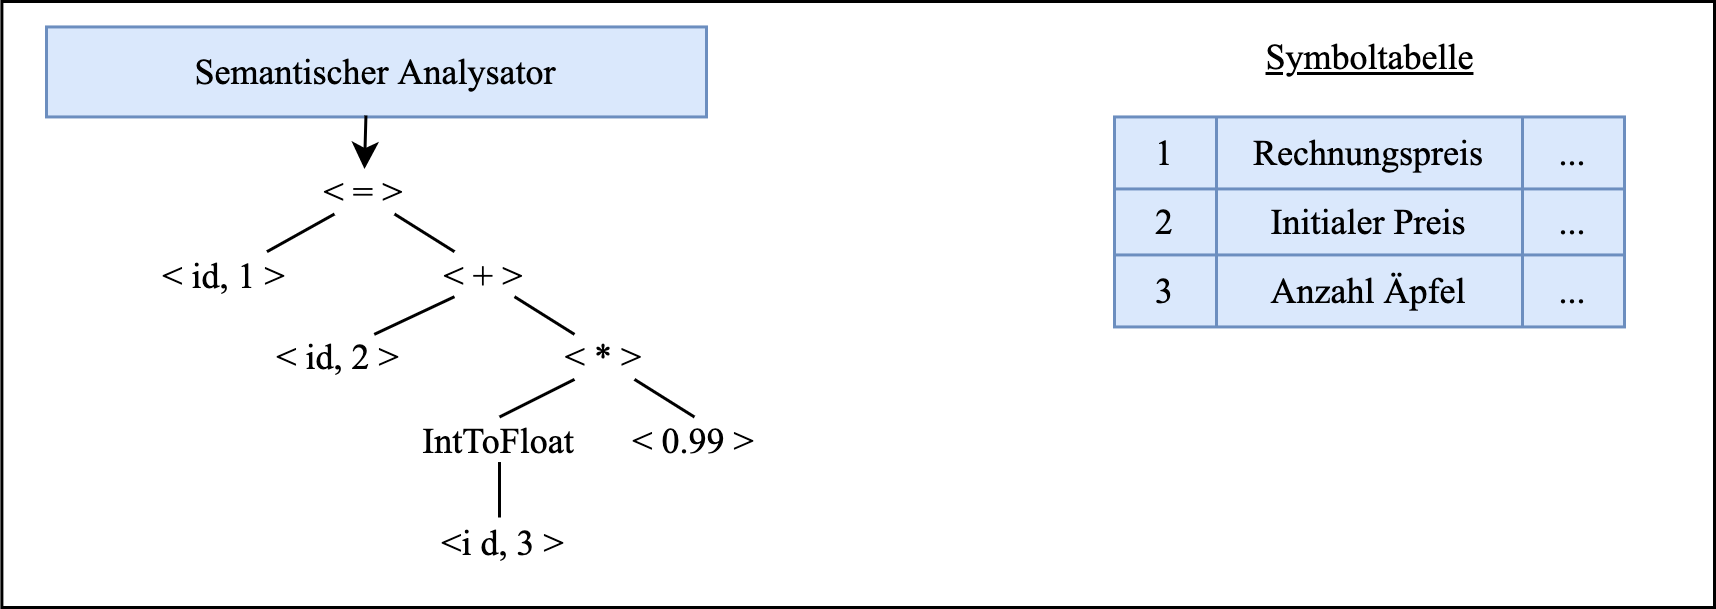
\includegraphics[width=\textwidth,keepaspectratio]{Images/Compiler/Type.png}
 \caption[Typüberprüfung]{Typüberprüfung \protect\footcite{Ullmann2008} }
 \label{fig:Typ}
\end{figure}
\footnotetext{Abbildung in Anlehnung an Ullman et al. 2008, S.10.} 
\section{Zwischencodeerzeugung}
Während der Übersetzung eines Programms  kann der Compiler mehrere Zwischendarstellungen in unterschiedlichsten Formen,  zum Beispiel wie die eines Syntaxbaums, erstellen.  
Nach der semantischen Analyse stellen viele Compiler eine maschinennahe Zwischendarstellung auf niedriger Abstraktionsebene her, die eigentlich für maschinenabhängige Aufgaben wie Befehlsauswahl geeignet ist. 
\begin{figure}[!ht]
 
\includegraphics[width=\textwidth,keepaspectratio]{Images/Compiler/Zwischendarstellungen.png}
 \caption[Zwischendarstellungen]{Zwischendarstellungen \protect\footcite{Ullmann2008} }
 \label{fig:Zwischendarstellung}
\end{figure}
\footnotetext{Abbildung in Anlehnung an Ullman et al. 2008, S.433.} 
Eine Zwischendarstellung, die von Compiler zu Compiler in Auswahl oder Entwurf unterschiedlich ist,  kann entweder eine tatsächliche Sprache sein,  oder aus internen Datenstrukturen bestehen, die von den Phasen des Compilers gemeinsam verwendet werden. Auch wenn C eine Programmiersprache ist, wird sie häufig als eine Zwischenform verwendet, da sie flexibel ist, zu effizientem Maschinencode kompiliert werden kann und ihre Compiler weitgehend verfügbar sind.\footcite[Vgl.][S. 433]{Ullmann2008}


\section{Codeoptimierung}
In dieser Phase wird der Code so optimiert, dass sich daraus ein besserer,  das heißt schnellerer oder ressourcenschonender Zielcode ergibt.  Der Umfang der Codeoptimierung schwankt dabei von Compiler zu Compiler erheblich.  \footcite[Vgl.][S. 11f]{Ullmann2008} 
Die Codeoptimierung, die ein Compiler vornimmt, ist im Laufe der Zeit wichtiger und  komplexer geworden. Grund für die zunehmende Komplexität sind die immer komplexeren Prozessorarchitekturen, die mehr Gelegenheiten bieten, die Ausführung des  Codes zu verbessern. Die gestiegene Bedeutung ergibt sich Beispielsweise aus der steigenden Anzahl an Kernen in modernen Computern und der Möglichkeit, Programme parallel auszuführen.\footcite[Vgl.][S. 20]{Ullmann2008}

\section{Codeerzeugung}
Die Überführung aus der Zwischendarstellung in die Zielsprache nennt man Codeerzeugung.  Hierbei muss die semantische Bedeutung des Quellprogramms erhalten und hochwertig dargestellt sein. Die größte Herausforderung ergibt sich aus der nicht komplett mathematischen Berechenbarkeit aller Prozesse bei der Überführung. Ein Beispiel wäre die Vergabe von Registern,  die nicht effizient berechenbar sind.  In der Praxis müssen heuristische Techniken ausreichen- die guten, aber nicht unbedingt optimalen Code liefern.  Die Codeoptimierungs- und  Codeerzeugungsphasen können mehrfach durchlaufen werden,  bevor das Zielprogramm finalisiert ist. \footcite[Vgl.][S. 618f]{Ullmann2008}

\section{Der .NET Compiler Roslyn}
Für die Arbeit mit der Programmiersprache \Csharp  steht mit Roslyn ein Compiler zur Verfügung, der sich aus modularen Bibliotheken zusammensetzt.  Durch die Referenzierung dieser Bibliotheken können Programme auf den Funktionsumfang von Roslyn zugreifen.  So ist es möglich, den Compiler zu verwenden, ohne das Ziel zu haben, die Programmiersprache \Csharp  in plattformnahen Code zu übersetzen.  Dabei stehen die Bibliotheken über den Packetmanager Nuget für die Einbindung in eigene Projekte zur Verfügung.  Um diese Funktionalität zu gewährleisten,  unterteilt Rosyln die Übersetzung in mehrere Phasen,  welche wiederum einige der in diesem Kapitel beschriebenen Phasen zusammenfassen. Die erste Phase ist die Erstellung des Syntaxbaums, die zweite Phase ist die semantische Analyse gefolgt von der letzten Phase der Ausgabe der so genannten Intermediate Language als Zielsprache. \footcite[Vgl.][S. 1017]{Albahari2020}




  \chapter{Cross Plattform Frameworks}
Für die Realisierung eine Source-to-Source Compilers gibt es zwei relevante Faktoren,  die für die Realisierung ausschlaggebend sind.  Zum einen die Programmiersprachen in dem die beiden Frameworks entwickelt werden,  da bei der Übersetzung eine Brücke zwischen Quell und Zielsprache geschlagen werden muss.  Neben der Programmiersprache ist jedoch auch die Arbeitsweise eines Frameworks von essentieller Bedeutung.  Wie die Definition von Compilern bereits einführte,  müssen die Programme vor und nach der Übersetzung gleichwertig sein.  Dies implementiert,  dass das Verhalten der übersetzten Anwendungen nach der Übersetzung identisch seien muss wie das der Ursprungsanwendung.  Es ist also notwendig,  neben den sprachlichen auch die technischen Unterschiede zwischen den Frameworks zu kennen und diese im Rahmen der compilierung zu optimieren. 

\section{Frameworks}
Xamarin is eine Open Source-Plattform für das Erstellen mobiler Anwendungen für iOS und Android mit Hilfe des .NET Frameworks, welches von Microsoft weiterentwickelt wird.  Dabei ist Xamarin ist eine Abstraktionsebene, die die Kommunikation zwischen Code und dem zugrunde liegenden Plattformcode verwaltet.  Xamarin wird in einer verwalteten Umgebung ausgeführt, die Vorteile wie Speicherbelegung und Garbage Collection bietet.  Bei Xamarin.Forms handelt es sich um ein Open-Source-Benutzeroberflächenframework., mit dessen Hilfe Entwickler iOS- und Android- Anwendungen aus einer einzigen CodeBase erstellen können.  Dabei wird auf die in der .NET Welt bekannten Technologien XAML  für die Benutzeroberfläche und C\# für die Anwendungslogik zurückgegriffen.  Die einzelnen Benutzeroberflächen werden von Xamarin.Forms als native Steuerelemente auf jeder Plattform gerendert.  \footcite[Vgl.][Abgerufen am \today]{MicrosoftWhatIsXam2020}

Flutter ist ebenfalls wie Xamarin.Forms ein Open Source Framework für die Erstellung von 2D mobilen Anwendungen.  Dabei werden im Vergleich zu Xamarin.Forms keine nativen Steuerelemente für jede Plattform gerendert sondern beinhaltet eine Sammlung von so genannten Widgets, die von dem Framework vewaltet und gerendert werden.  Für die Anzeige dieser Widgets wird auf die 2D engine Skia zugegriffen.  Flutter geht diesen Weg,  da das Endergebnis der Anwendungen eine höhere Qualität verspricht, da die nativen Steuerelemente in Bezug auf Flexibilität und Qualität begrenzt sind.  Außerdem ist es durch die Verwendung derselben Renderes einfacher, von derselben Codebasis aus für mehrere Plattformen zu veröffentlichen,  ohne eine sorgfältige und kostspielige Planung vornehmen zu müssen,  um verschiedene Funktionssätze und API-Merkmale aufeinander abzustimmen.\footcite[Vgl.][Abgerufen am \today]{GoogleFlutterFAQ2020}

Dieser essentielle Unterschied zwischen den Frameworks werden in den folgenden Abschnitten dieser Arbeit deutlicher und sind bei der Übersetzung der Anwendungen fokussiert zu Berücksichtigen. 
\subsection{Projekte}
Xamarin.Forms Projektmappen setzen sich aus mehreren Projekten zusammen., jeweils eins für die Plattform (iOS/ Android),  welche den plattformspezifischen Code und assets in Form von Icons und Metadaten beinhalten sowie ein zusätzliches für den Quelltext,  der zwischen den Plattformen geteilt wird.  \footcite[Vgl.][S. 25f.]{Petzold2016} Im Gegensatz dazu gibt es bei Flutter nur ein Projekt, welches alle notwendigen Inhalte für iOS und Android beinhaltet.  Für plattformspezifischen Code gibt es jeweils einen Ordner für iOS und Android. \footcite[Vgl.][S. 113]{Biessek2019}

\subsection{Views}
Views (zu Deutsch Ansichten) sind visuelle Elemente die in zwei Kategorien unterschieden werden können.  Controls, die für die Sammlung von Benutzereingaben oder die Ausgabe von Daten sind.  Sowie Layouts die eine Sammlung von Ansichten beinhalten und für die Anordnung der untergeorderten Ansichten in der Benutzeroberfläche verantwortlich sind.  Außerdem arbeitet sie mit jeder untergeordneten Ansicht zusammen, um die endgültige Rendering-Größe zu bestimmen.\footcite[Vgl.][Abgerufen am \today]{Ritscher2020}
\subsubsection{Pages}
Pages (zu Deutsch: Ansichtseiten) sind visuelle Elemente einer Anwendung die den gesamten Bildschirm belegen und zu den Layout Views gehören.  Xamarin Forms bietet dafür 
verschiedene Alternativen an,  die in \ref{fig:Xamarin.Forms Pages} grafisch dargestellt sind.\footcite[Vgl.][Abgerufen am \today]{MicrosoftXamPages2016}

\begin{figure}[h]
 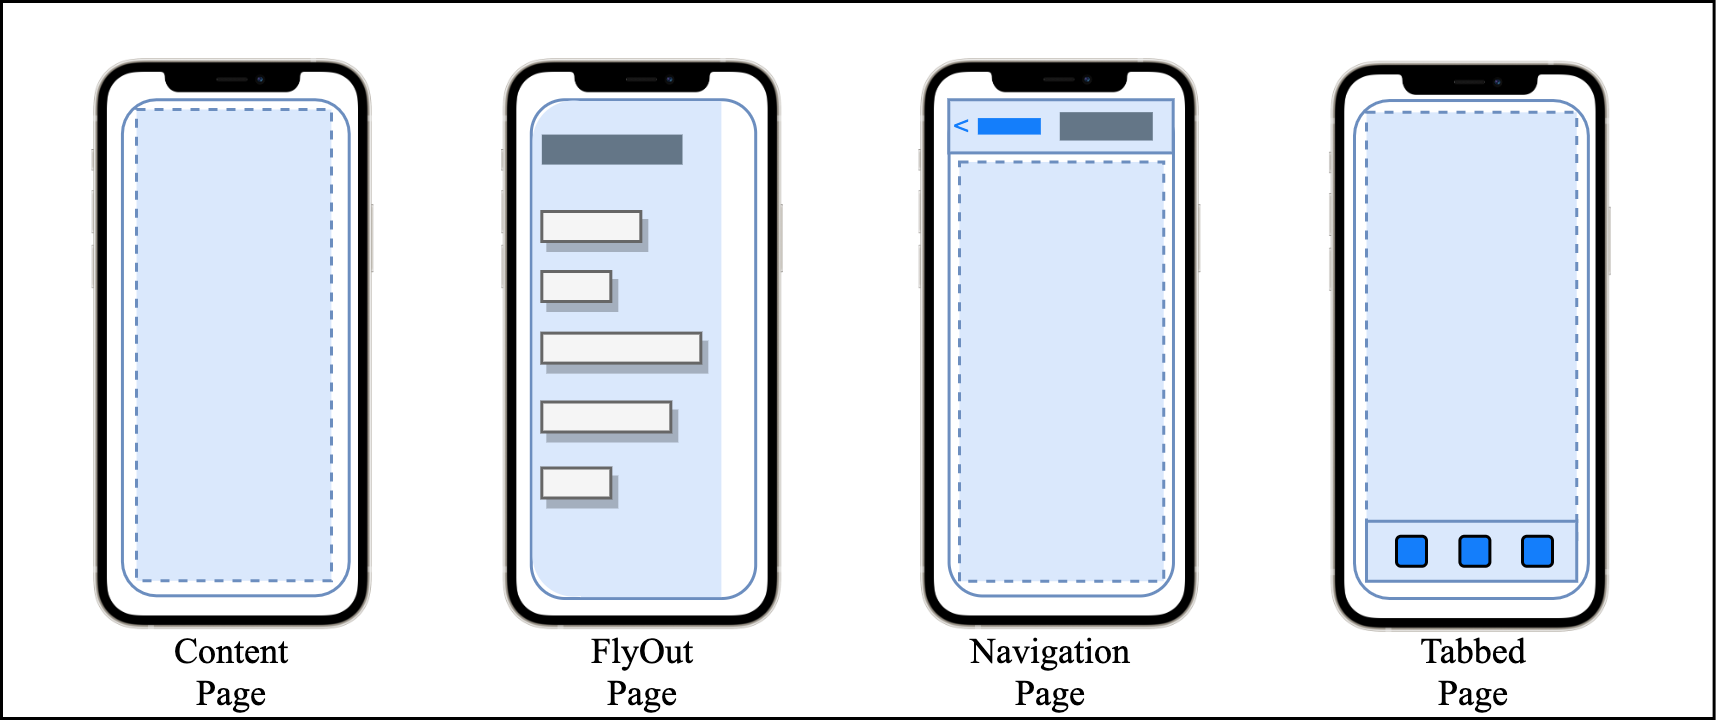
\includegraphics[width=\textwidth,height=\textheight,keepaspectratio]{Images/CrossPlattformFrameworks/XamarinFormsPages.png}
 \caption[Xamarin.Forms Pages]{Xamarin.Forms Pages\footnotemark}
 \label{fig:Xamarin.Forms Pages}
\end{figure}
\footcitetext[Abbildung in Anlehnung an ][Abgerufen am \today]{MicrosoftXamPages2016}
Wie die Darstellung präsentiert, hat die Auswahl einer Page einen direkten Einfluss auf das Navigationskonzept innerhalb der Anwendung.  Abgesehen von der ContentPage, die ausschließlich eine View anzeigt haben die jeweiligen Seiten das folgende Navigationskonzept: \footcite[Vgl.][Abgerufen am \today]{MicrosoftXamPages2016}

\begin{itemize}
\setlength\itemsep{-0.6em}
 \item FlyOutPage: Eine Seite, die zwei Bereiche für die Seite hat. Typischerweise enthält das Flyout ein Menü über welches zwischen den eigentlichen Inhaltsseiten navigiert werden kann.
 \item NavigationPage: Eine Seite,  die eine Navigationsleiste enthält.  Die Seiten werden auf einem Stapel gehalten und es kann zwischen ihnen gesprungen werden.  Die Navigationsleiste kann sowohl Navigationsschaltflächen als auch einen Titel enthalten.
 \item TabbedPage: Eine Container-Seite.  Die TabbedPage fungiert als Container,  der die mit jeder Registerkarte verbundenen Inhaltsseiten enthält.
\end{itemize}

Die Auswahl einer Page wird innerhalb des Wurzelknoten der XAML Datei definiert.  Dies wird in Quelltext \ref{lst:TabbedPage} dargestellt. 

\begin{minipage}{\linewidth}
\lstinputlisting[label={lst:TabbedPage},caption={Xamarin.Forms TabbedPage definition}, language=XML]{SourceCode/XamarinFormsTabbedPage.XAML}
\end{minipage}

Das Beispiel zeigt eine TabbedPage mit drei in diesem Falle leeren NavigationsPages die als Children der TabbedPage hinzugefügt werden.  Im Gegensatz zu der TabbedPage hat die FlyoutPage keine Sammlung von ChildrenPages sondern ein sogenanntes "Flyout" welches das Menu beinhaltet und die entsprechend ausgewählte Seite in eine Detailansicht läd.  Dies wird in Quelltext \ref{lst:FlyOutPage} dargestellt.

\begin{minipage}{\linewidth}
\lstinputlisting[label={lst:FlyOutPage},caption={Xamarin.Forms FlyOut definition}, language=XML]{SourceCode/XamarinFormsFlyoutPage.XAML}
\end{minipage}

Im Gegensatz zu Xamarin.Forms lässt sich bei Flutter auf der Ebene der Wurzel kein Navigationskonzept definieren,  sondern ausschließlich das Style der Anwendung.  Flutter unterstützt drei alternativen: MaterialApp erzeugt eine App mit dem von Google entwickelten Material Design, CupertinoApp für eine App im iOS-Stil oder die Definition eines eigenen Styles für eine individuelle Anzeige.  \footcite[Vgl.][Abgerufen am \today]{GoogleFlutterPages2020}  Quelltext \ref{lst:MaterialApp} zeigt die Definition einer MaterialDesign App in Flutter.

\begin{minipage}{\linewidth}
\lstinputlisting[label={lst:MaterialApp},caption={Flutter MaterialApp definition}, language=Dart]{SourceCode/MaterialApp.Dart}
\end{minipage}

Von diesem Widget aus ist die eigentliche erste Seite ein weiteres zustandsabhängiges Widget.  Dieses besteht aus zwei Teilen:  Der erste Teil, der selbst unveränderlich ist, erzeugt ein State-Objekt, das den Zustand des Objekts enthält.  Das State-Objekt bleibt während der Lebensdauer des Widgets bestehen. Das State-Objekt implementiert die build()-Methode für das zustandsabhängige Widget.  Wenn sich der Zustand des Widget-Baums ändert,  wird setState() aufgerufen was einen Build des entsprechenden Teils der Benutzeroberfläche auslöst.  In Flutter ist die Benutzeroberfläche (auch bekannt als Widget-Baum) unveränderlich,  dass bedeutet da der Zustand nicht mehr geändert werden kann, sobald dieser aufgebaut ist.  Sie ändern Felder in Ihrer State-Klasse und rufen dann setState() auf, um den gesamten Widget-Baum neu zu erstellen. \footcite[Vgl.][Abgerufen am \today]{GoogleFlutterSharedPreferences2020} 

Damit die Navigation ähnlich wie in Xamarin.Forms definiert werden kann müssen verschiedene Widgets in einem Widget Baum verschachtelt werden.  Quelltext \ref{lst:FlutterTabbedApp} zeigt dies für die Arbeit mit Tabbs.  In diesem Beispiel wird eine TabBar mit drei Tab-Widgets erstellt und diese innerhalb einer AppBar platziert.\footcite[Vgl.][Abgerufen am \today]{GoogleFlutterTabs2020} 


\begin{minipage}{\linewidth}
\lstinputlisting[label={lst:FlutterTabbedApp},caption={Flutter Tab Layout definition}, language=Dart]{SourceCode/TabbedPage.Dart}
\end{minipage}


\subsubsection{Layouts}

Layouts werden in Xamarin.Forms verwendet, um die Steuerelemente der Benutzeroberfläche zu visuellen Strukturen zusammenzustellen. Dabei unterscheidet man zwischen Layouts die ausschließlich einen oder mehrere Inhalte beinhalten können.  Xamarin.Forms bietet die folgende Layouts an:\footcite[Vgl.][Abgerufen am \today]{MicrosoftXamLayouts2018} 


\begin{itemize}
\setlength\itemsep{-0.6em}
 \item ContentView: ContentView enthält ein einzelnes untergeordnetes Element, das mit der Eigenschaft "Content" festgelegt wird. Die Eigenschaft Content kann auf jedes View-Derivat gesetzt werden, auch auf andere Layout-Derivate. ContentView wird meist als Strukturelement verwendet und dient als Basisklasse zu Frame.
 \item Frame: Die Klasse Frame leitet sich von ContentView ab und zeigt einen Rahmen um die Ansicht.
  \item ScrollView: Ist in der Lage, seinen Inhalt zu scrollen.  Die Eigenschaft Content auf eine Ansicht oder ein Layout fest, das zu groß ist, um auf den Bildschirm zu passen.  Legen Sie die Eigenschaft Orientierung fest, um anzugeben, ob der Bildlauf vertikal, horizontal oder beides sein soll.
 \item StackLayout: Positioniert untergeordnete Elemente in einem Stapel entweder horizontal oder vertikal, basierend auf der Eigenschaft Orientation.
 \item Grid: Grid positioniert seine untergeordneten Elemente in einem Raster aus Zeilen und Spalten. Die Position eines untergeordneten Elements wird über die angehängten Eigenschaften Row, Column, RowSpan und ColumnSpan angegeben.
 \item AbsolutLayout: Positioniert untergeordnete Elemente an bestimmten Positionen relativ zu ihrem übergeordneten Element. Die Position eines untergeordneten Elements wird über die angehängten Eigenschaften LayoutBounds und LayoutFlags angegeben. Ein AbsoluteLayout ist nützlich, um die Positionen von Ansichten zu animieren.
 \item RelativeLayout:  Positioniert untergeordnete Elemente relativ zum RelativeLayout selbst oder zu ihren Geschwistern. Die Position eines Kindelements wird über die angehängten Eigenschaften angegeben, die auf Objekte vom Typ Constraint und BoundsConstraint gesetzt werden.
\end{itemize}

Alle verfügbaren Layouts werden in  \ref{fig:Xamarin.Forms Layouts} grafisch dargestellt.

\begin{figure}[h]
 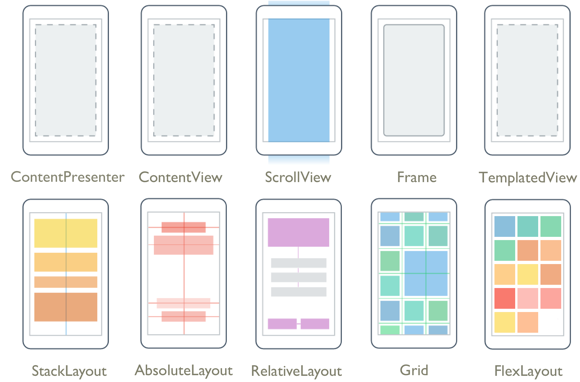
\includegraphics[width=\textwidth,height=\textheight,keepaspectratio]{Images/CrossPlattformFrameworks/XamarinFormsLayouts.png}
 \caption[Xamarin.Forms Layouts]{Xamarin.Forms Layouts\footnotemark}
 \label{fig:Xamarin.Forms Layouts}
\end{figure}
\footcitetext[Abbildung in Anlehnung an ][Abgerufen am \today]{MicrosoftXamLayouts2018}


\subsubsection{Steuerelemente}

Xamarin.Forms-Ansichten sind die Bausteine von plattformübergreifenden mobilen Benutzeroberflächen. Ansichten sind Objekte der Benutzeroberfläche wie Beschriftungen, Schaltflächen und Schieberegler, die in anderen grafischen Programmierumgebungen üblicherweise als Steuerelemente oder Widgets bezeichnet werden. Die von Xamarin.Forms unterstützten Ansichten leiten sich alle von der Klasse View ab. 
\subsubsection{Steuerelemente für die Darstellung}

\begin{itemize}
\setlength\itemsep{-0.6em}
 \item BoxView zeigt ein einfarbiges Rechteck an 
 \item Ellipse zeigt eine Ellipse oder einen Kreis an
  \item Label zeigt einzeilige Textstrings oder mehrzeilige Textblöcke an, entweder mit konstanter oder variabler Formatierung.
 \item Line zeigt eine Linie von einem Startpunkt zu einem Endpunkt an
 \item Image zeigt ein Bitmap an, diese können über das Web heruntergeladen, als Ressourcen in über das gemeinsame Projekt oder in Plattformprojekte eingebettet  werden
 \item Map zeigt eine Karte an
 \item OpenGLView zeigt OpenGL-Grafiken an
 \item Path zeigt Kurven und komplexe Formen an.
 \item Polygon Polygon zeigt ein Polygon an.
 \item  Polyline zeigt eine Reihe von verbundenen geraden Linien an
 \item Rectangle zeigt ein Rechteck oder Quadrat an
 \item WebView zeigt Web-Seiten oder HTML-Inhalte an
\end{itemize}

\subsubsection{Steuerelemente die Aktionen auslösen}

\begin{itemize}
\setlength\itemsep{-0.6em}
 \item Button ist ein rechteckiges Objekt, das Text anzeigt und ein Clicked-Ereignis auslöst, wenn es gedrückt wurde.
 \item ImageButton ist ein rechteckiges Objekt, das ein Bild anzeigt und ein Clicked-Ereignis auslöst, wenn es gedrückt wurde.
  \item RadioButton erlaubt die Auswahl einer Option aus einer Menge und feuert ein CheckedChanged-Ereignis, wenn die Auswahl erfolgt.
 \item RefreshView ist ein Container-Steuerelement, das eine Pull-to-Refresh-Funktionalität für scrollbare Inhalte bietet. 
 \item SearchBar zeigt einen Bereich an, in dem der Benutzer eine Textzeichenfolge eingeben kann, sowie eine Schaltfläche (oder eine Tastaturtaste), die der Anwendung signalisiert, eine Suche durchzuführen
 \item SwipeView ist ein Container-Steuerelement, das sich um ein Inhaltselement legt und Kontextmenüelemente bereitstellt, die durch eine Wischgeste angezeigt werden
\end{itemize}



\subsubsection{Steuerelemente um Werte zu setzen}


\begin{itemize}
\setlength\itemsep{-0.6em}
 \item CheckBox ermöglicht dem Benutzer die Auswahl eines booleschen Wertes mit Hilfe einer Art Schaltfläche, die entweder markiert oder leer sein kann
 \item Schieberegler bieten Benutzern die Option einen  Wert aus einem kontinuierlichen Bereich auswählen, der mit den Eigenschaften Minimum und Maximum festgelegt wurde.
 \item Stepper ermöglicht es dem Benutzer, einen doppelten Wert aus einem Bereich von inkrementellen Werten auszuwählen, die mit den Eigenschaften Minimum, Maximum und Inkrement festgelegt wurden.
 \item Schalter hat die Form eines Ein/Aus-Schalters, damit der Benutzer einen booleschen Wert auswählen kann
 \item DatePicker ermöglicht es dem Benutzer, ein Datum mit der Datumsauswahl der Plattform auszuwählen.
 \item TimePicker ermöglicht dem Benutzer die Auswahl einer Zeit mit dem TimePicker der Plattform
\end{itemize}
\subsubsection{Steuerelemente um text zu manipulieren}

\begin{itemize}
\setlength\itemsep{-0.6em}
 \item Entry ermöglicht dem Benutzer die Eingabe und Bearbeitung einer einzelnen Textzeile
 \item Editor ermöglicht dem Benutzer die Eingabe und Bearbeitung mehrerer Textzeilen
\end{itemize}
\subsubsection{Steuerelemente um eine Aktivität anzudeuten}


\begin{itemize}
\setlength\itemsep{-0.6em}
 \item ActivityIndicator verwendet eine Animation, um zu zeigen, dass die Anwendung eine langwierige Aktivität ausführt, ohne einen Hinweis auf den Fortschritt zu geben. 
 \item ProgressBar verwendet eine Animation, um zu zeigen, dass die Anwendung durch eine langwierige Aktivität fortschreitet
\end{itemize}

\subsubsection{Steuerelemente um Sammlungen anzuzeigen}
\begin{itemize}
\setlength\itemsep{-0.6em}
 \item CarouselView zeigt eine blätterbare Liste von Datenelementen an
 \item CollectionView zeigt eine scrollbare Liste mit auswählbaren Datenelementen an, wobei verschiedene Layout-Spezifikationen verwendet werden. Sie soll eine flexiblere und performantere Alternative zu ListView darstellen. 
  \item IndicatorView zeigt Indikatoren an, die die Anzahl der Elemente in einer CarouselView darstellen
 \item ListView zeigt eine scrollbare Liste mit auswählbaren Datenelementen an
 \item Picker zeigt ein ausgewähltes Element aus einer Liste von Textzeichenfolgen an und ermöglicht die Auswahl dieses Elements, wenn die Ansicht angetippt wird
 \item TableView zeigt eine Liste von Zeilen mit optionalen Überschriften und Unterüberschriften an
\end{itemize}

\subsubsection{Listen}
\subsubsection{Gesten}
\subsubsection{Animtion}

\subsection{Navigation}
In Xamarin.Forms bietet die Klasse NavigationPage eine hierarchische Navigation, bei der der Benutzer durch die Seiten, vorwärts und rückwärts, navigieren kann.

Flutter hat eine ähnliche Implementierung, die einen Navigator und Routen verwendet. Eine Route ist eine Abstraktion für eine Seite einer App, und ein Navigator ist ein Widget, das Routen verwaltet. Eine Route bildet grob eine Seite ab. Der Navigator arbeitet ähnlich wie die Xamarin.Forms NavigationPage, indem er Routen push() und pop() kann, je nachdem, ob man zu einer Ansicht hin oder von ihr zurück navigieren möchte.

\subsubsection{Navigation zu anderen Apps}
In Xamarin.Forms verwenden kann, um zu einer anderen Anwendung zu navigieren, ein bestimmtes URI-Schema verwendet werden.  So z.B. mit dem Befehl Device.OpenUrl("mailto://") das Standard E-Mail-Programm des Gerätes geöffnet werden verwenden.
Um diese Funktionalität in Flutter zu implementieren,  muss eine native Plattformintegration oder eine vorhandenes Plugin, wie z. B. urllauncher verwendet werden.  
\subsection{Async UI}
Dart hat ein Single-Thread-Ausführungsmodell mit Unterstützung für Isolates (eine Möglichkeit, Dart-Code in einem anderen Thread auszuführen), eine Ereignisschleife und asynchrone Programmierung. Sofern Sie kein Isolate erzeugen, wird Ihr Dart-Code im Haupt-Thread der Benutzeroberfläche ausgeführt und von einer Ereignisschleife gesteuert.

Das Single-Thread-Modell von Dart bedeutet nicht, dass Sie alles als blockierende Operation ausführen müssen, die das Einfrieren der Benutzeroberfläche verursacht. Ähnlich wie bei Xamarin.Forms müssen Sie den UI-Thread frei halten. Sie würden async/await verwenden, um Aufgaben auszuführen, bei denen Sie auf die Antwort warten müssen.

In Flutter verwenden Sie die asynchronen Möglichkeiten, die die Sprache Dart bietet, auch async await genannt, um asynchrone Arbeiten auszuführen. Dies ist C\# sehr ähnlich und sollte für jeden Xamarin.Forms-Entwickler sehr einfach zu verwenden sein.

Sie können zum Beispiel Netzwerkcode ausführen, ohne dass die Benutzeroberfläche hängen bleibt, indem Sie async await verwenden und Dart die schwere Arbeit erledigen lassen:
Sobald der erwartete Netzwerkaufruf erfolgt ist, aktualisieren Sie die Benutzeroberfläche durch den Aufruf von setState(), was einen Neuaufbau des Widget-Unterbaums auslöst und die Daten aktualisiert.
\subsection{Hintergrundarbeiten}
Da Flutter Single-Thread-fähig ist und eine Ereignisschleife ausführt, müssen Sie sich nicht um das Thread-Management oder das Erzeugen von Hintergrund-Threads kümmern. Dies ist sehr ähnlich wie bei Xamarin.Forms. Wenn Sie E A-gebundene Arbeiten durchführen, wie z. B. Festplattenzugriffe oder Netzwerkaufrufe, dann können Sie async await verwenden und alles ist bereit.

Wenn Sie andererseits rechenintensive Arbeiten ausführen müssen, die die CPU beschäftigen, sollten Sie sie in ein Isolate verschieben, um ein Blockieren der Ereignisschleife zu vermeiden, so wie Sie jede Art von Arbeit aus dem Hauptthread heraushalten würden. Dies ist ähnlich, wie wenn Sie Dinge über Task.Run() in Xamarin.Forms in einen anderen Thread verschieben.

Für E/A-gebundene Arbeit deklarieren Sie die Funktion als asynchrone Funktion und warten Sie auf lang laufende Aufgaben innerhalb der Funktion.

So würden Sie normalerweise Netzwerk- oder Datenbankaufrufe durchführen, die beide E/A-Operationen sind.

Es kann jedoch vorkommen, dass Sie eine große Datenmenge verarbeiten und Ihre Benutzeroberfläche hängen bleibt. In Flutter verwenden Sie Isolates, um die Vorteile mehrerer CPU-Kerne zu nutzen, um langlaufende oder rechenintensive Aufgaben zu erledigen.

Isolates sind separate Ausführungsthreads, die sich keinen Speicher mit dem Hauptspeicherheap der Ausführung teilen. Dies ist ein Unterschied zu Task.Run(). Das bedeutet, dass Sie vom Haupt-Thread aus nicht auf Variablen zugreifen oder Ihre Benutzeroberfläche durch den Aufruf von setState() aktualisieren können.
\subsection{Netzwerkaufrufe}
In Xamarin.Forms würden Sie HttpClient verwenden. Einen Netzwerkaufruf in Flutter zu machen ist einfach, wenn Sie das beliebte http-Paket verwenden. Dieses abstrahiert einen Großteil des Netzwerks, das Sie normalerweise selbst implementieren würden, und macht es einfach, Netzwerkaufrufe zu tätigen.

Um das http-Paket zu verwenden, fügen Sie es zu Ihren Abhängigkeiten in pubspec.yaml hinzu.

Um eine Netzwerkanfrage zu stellen, rufen Sie await auf die asynchrone Funktion wie in \ref{lst:FlutterNetworkRequest} dargestellt auf:


\begin{minipage}{\linewidth}
\lstinputlisting[label={lst:FlutterNetworkRequest},caption={Flutter Network request}, language=Dart]{SourceCode/NetworkRequest.Dart}
\end{minipage}

\subsection{Lebenzyklus}
In Xamarin.Forms haben Sie eine Anwendung, die OnStart, OnResume und OnSleep enthält. In Flutter können Sie stattdessen auf ähnliche Lebenszyklusereignisse hören, indem Sie sich in den WidgetsBinding-Beobachter einklinken und auf das Änderungsereignis didChangeAppLifecycleState() hören.

Die beobachtbaren Lebenszyklus-Ereignisse sind:

`inactive`
Die Anwendung befindet sich in einem inaktiven Zustand und empfängt keine Benutzereingaben. Dieses Ereignis ist nur für iOS verfügbar.
`paused`
Die Anwendung ist derzeit für den Benutzer nicht sichtbar, reagiert nicht auf Benutzereingaben, wird aber im Hintergrund ausgeführt.
Wiederaufgenommen
Die Anwendung ist sichtbar und reagiert auf Benutzereingaben.
Suspendiert
Die Anwendung ist momentan angehalten. Dieses Ereignis ist nur für Android verfügbar.
\subsection{Bilder}
Flutter folgt einem einfachen dichtebasierten Format wie iOS. Assets können 1,0x, 2,0x, 3,0x oder ein anderer Multiplikator sein. Flutter hat keine dps, aber es gibt logische Pixel, die im Grunde dasselbe sind wie geräteunabhängige Pixel. Das sogenannte devicePixelRatio drückt das Verhältnis von physikalischen Pixeln zu einem einzelnen logischen Pixel aus.

Assets befinden sich in einem beliebigen Ordner - Flutter hat keine vordefinierte Ordnerstruktur. Sie deklarieren die Assets (mit Speicherort) in der Datei pubspec.yaml, und Flutter holt sie ab.

Beachten Sie, dass vor Flutter 1.0 beta 2 die in Flutter definierten Assets nicht von der nativen Seite aus zugänglich waren, und umgekehrt waren die nativen Assets und Ressourcen für Flutter nicht verfügbar, da sie in separaten Ordnern lagen.

Ab Flutter Beta 2 werden die Assets im nativen Asset-Ordner gespeichert und auf der nativen Seite über den AssetManager von Android aufgerufen:

Ab Flutter beta 2 kann Flutter immer noch nicht auf native Ressourcen zugreifen, noch kann es auf native Assets zugreifen.

Um zum Beispiel ein neues Bild-Asset mit dem Namen myicon.png zu unserem Flutter-Projekt hinzuzufügen und zu entscheiden, dass es in einem Ordner liegen soll, den wir willkürlich images genannt haben, würden Sie das Basisbild (1.0x) in den images-Ordner legen und alle anderen Varianten in Unterordnern, die mit dem entsprechenden Verhältnismultiplikator genannt werden:
\subsection{Schriften}
In Xamarin.Forms müssten Sie in jedem nativen Projekt eine eigene Schriftart hinzufügen. Dann würden Sie in Ihrem Element diesen Schriftnamen dem FontFamily-Attribut zuweisen, indem Sie filenamefontname und nur fontname für iOS verwenden.

In Flutter legen Sie die Schriftdatei in einem Ordner ab und referenzieren sie in der Datei pubspec.yaml, ähnlich wie Sie Bilder importieren.
Weisen Sie dann die Schriftart Ihrem Text-Widget zu, wie in  \ref{lst:FlutterFont} dargestellt. 

\begin{minipage}{\linewidth}
\lstinputlisting[label={lst:FlutterFont},caption={Flutter Font definition}, language=Dart]{SourceCode/Fonts.Dart}
\end{minipage}

\subsection{Plugins}
Im .NET-Ökosystem können native Xamarin-Projekte und Xamarin.Forms-Projekte Zugriff auf Nuget und das eingebaute Paketverwaltungssystem zurrückgreifen um.  Flutter-Apps enthalten eine native Android-App, eine native iOS-App und eine Flutter-App.
In Android fügen Sie Abhängigkeiten hinzu, indem Sie Ihr Gradle-Build-Skript ergänzen. In iOS fügen Sie Abhängigkeiten hinzu, indem Sie Ihr Podfile hinzufügen.
Flutter verwendet das eigene Build-System von Dart und den Pub-Paketmanager. Die Werkzeuge delegieren die Erstellung der nativen Android- und iOS-Wrapper-Apps an die jeweiligen Build-Systeme.
Generell sollten das pubspec.yaml verwendet werden, um externe Abhängigkeiten zu deklarieren, die in Flutter verwendet werden sollen. Ein guter Ort, um Flutter-Pakete zu finden, ist auf pub.dev.

\subsection{Interaktion mit der Hardware}

Flutter führt den Code nicht direkt auf der zugrundeliegenden Plattform aus. Vielmehr wird der Dart-Code, aus dem eine Flutter-App besteht, nativ auf dem Gerät ausgeführt, wobei das von der Plattform bereitgestellte SDK "umgangen" wird. Das bedeutet, wenn Sie zum Beispiel eine Netzwerkanfrage in Dart durchführen, wird diese direkt im Dart-Kontext ausgeführt. Sie verwenden nicht die Android- oder iOS-APIs, die Sie normalerweise beim Schreiben nativer Apps nutzen. Ihre Flutter-App wird immer noch im ViewController oder der Activity einer nativen App als View gehostet, aber Sie haben keinen direkten Zugriff auf diesen oder das native Framework.

Das bedeutet aber nicht, dass Flutter-Apps nicht mit diesen nativen APIs oder mit Ihrem nativen Code interagieren können. Flutter bietet Plattformkanäle, die mit dem ViewController oder der Activity, die Ihre Flutter-Ansicht hostet, kommunizieren und Daten austauschen. Plattformkanäle sind im Wesentlichen ein asynchroner Messaging-Mechanismus, der den Dart-Code mit dem Host-ViewController oder der Activity und dem iOS- oder Android-Framework, auf dem er läuft, verbindet. Sie können Plattformkanäle verwenden, um eine Methode auf der nativen Seite auszuführen oder um z. B. einige Daten von den Sensoren des Geräts abzurufen.

Zusätzlich zur direkten Verwendung von Plattformkanälen können Sie eine Vielzahl von vorgefertigten Plugins verwenden, die den nativen und Dart-Code für ein bestimmtes Ziel kapseln. Zum Beispiel können Sie ein Plugin verwenden, um auf die Kamerarolle und die Gerätekamera direkt von Flutter aus zuzugreifen, ohne eine eigene Integration schreiben zu müssen. Plugins finden Sie auf pub.dev, dem Open-Source-Paket-Repository von Dart und Flutter. Einige Pakete unterstützen möglicherweise native Integrationen auf iOS oder Android oder beides.

Wenn Sie kein Plugin auf pub.dev finden, das Ihren Anforderungen entspricht, können Sie Ihr eigenes schreiben und es auf pub.dev veröffentlichen.


\subsection{Storage}
Ein wesentlicher Bestandteil jeder mobilen Anwendung ist die Fähigkeit,  Daten zu persistieren.  Manchmal handelt es sich dabei um große Datenmengen,  die eine Datenbank erfordern,  oft sind es aber auch kleinere Daten wie Einstellungen und Präferenzen, die zwischen den Starts der Anwendung persistiert werden müssen.   
Xamarin.Essentials stellt Entwicklern plattformübergreifende APIs für ihre mobilen Anwendungen bereit,  indem es die einzigartigen Betriebssystem- und Plattform-APIs nativ anspricht. \footcite[Vgl.][Abgerufen am \today]{MicrosoftXamEssentials2020} In diesem Paket ist das Settingsplugin, welches die Speicherung von Einstellungen in einem Schlüsselwertspeicher erlaubt.  \footcite[Vgl.][Abgerufen am \today]{MicrosoftXamSettings2019} In Flutter wird für die Speicherung von Schlüssel-Wertpaaren auf die gleichen plattformspezifischen APIs zugegriffen wie bei Xamarin Forms diese werden mithilfe eines Plugins angesprochen.  \footcite[Vgl.][Abgerufen am \today]{GoogleFlutterSharedPreferences2020} 

Für die Speicherung in einer Datenbank können Xamarin.Forms Entwickler auf verschiedene Lösungen zurückgreifen zum einen SQLite  die am häufigsten verwendete Datenbank-Engine der Welt\footcite[Vgl.][Abgerufen am \today]{SQLiteConsortium2020},  oder Realm einer Datenbank optimiert für mobile Endgeräte. \footcite[Vgl.][Abgerufen am \today]{MongoDBRealm2020} Beide Datenbanken stehen auch als Plugin für Flutter zur Verfügung, wobei SQLite ausgereift ist,\footcite[Vgl.][Abgerufen am \today]{Tekartik2020} während Realm erst am 5 November 2020 support für Flutter angekündigt hat und noch nicht offiziell zur Verfügung steht. \footcite[Vgl.][Abgerufen am \today]{MongoDBFlutterSupport2020}


\section{Programmiersprachen}
C\# Dart Vergleich
XAML Dart


  %\chapter{Compiler Entwurf}

\section{Darstellung}
\section{CSharp to Dart}
\subsection{Variablen}
\subsection{Kontrollstrukturen}
\subsection{Framework Calls}

\section{XAML to Dart}
\subsection{Layouts}
\subsection{Steuerelemente}

\section{Ressourcen}
\subsection{Bilder}
\subsection{Fonts}

  
  %\chapter{Realisierung}
\label{chap:Realisierung}


\section{Umgebung}
Für die Realisierung und Verwendung des Compilers ist es notwendig verschiedene Softwarekomponenten erforderlich,  die an dieser Stelle mit Ihrer Funktion definiert werde sollen. 

\begin{itemize}
\setlength\itemsep{-0.6em}
 \item Windows 10:\footnote{Windows 10 ist über \url{https://www.microsoft.com/de-de/software-download/windows10ISO} zum download verfügbar. } Windows wird als Platform für den Übersetzer zwangsläufig benötigt, da der Roslyn Compiler ausschließlich für dieses Betriebssystem zur Verfügung steht. 
 \item Visual Studio 2019\footnote{Visual Studio 2019 ist über \url{https://visualstudio.microsoft.com/de/downloads/} zum download verfügbar. }: Die Entwicklungsumgebung für die Entwicklung des Übersetzers.  Mit Hilfe von Visual Studio kann ein Projekt angelegt werden,  welches den Roslyn Compiler verwenden kann.  Darüber hinaus kann mit Visual Studio eine Xamarin.Forms Anwendung entwickelt werden,  die für die spätere Qualitätssicherung des Übersetzers essentiell ist.  
 \item Build tools for Visual Studio:\footnote{Build tools for Visual Studio ist über \url{https://visualstudio.microsoft.com/de/downloads/} zum download verfügbar. } Beinhaltet MSBuild als teil der Build-Tool, das hilft, den Prozess der Erstellung eines Softwareprodukts zu automatisieren, einschließlich der Kompilierung des Quellcodes, der Paketierung, des Testens, der Bereitstellung und der Erstellung von Dokumentationen.  Mit MSBuild ist es möglich, Visual Studio-Projekte und -Lösungen zu erstellen, ohne dass die Visual Studio IDE installiert ist.
 \item Android Studio\footnote{Android Studio ist über \url{https://developer.android.com/studio} zum download verfügbar. } oder Visual Studio Code\footnote{ Visual Studio Code  ist über \url{https://code.visualstudio.com/} zum download verfügbar. }: Dabei handelt es sich um die Entwicklungsumgebungen für die Entwicklung von Flutter.  Für beide Umgebungen steht jeweils eine Erweiterung für die Programmiersprache Dart und das Flutter Framework bereit, die für die Arbeit mit Flutter Apps notwendig sind.  Im Rahmen dieser Arbeit ist eine dieser Umgebungen notwendig um die übersetzte Anwendung auszuführen. 
 \item Flutter SDK: \footnote{Die Flutter SDK ist über \url{https://flutter.dev/docs/get-started/install/windows} zum download verfügbar. } Das Flutter Software Development Kit (SDK)enthält die Pakete und Kommandozeilen-Tools, die Sie für die plattformübergreifende Entwicklung von Flutter-Apps benötigt werden. 
\end{itemize}




In der Zukunft könnte der Source to Source Compiler auch eine Web-Oberfläche bekommen,  diese hätte die zwei folgenden essentielle Vorteile im Gegensatz zu der aktuellen Implementierung.  Reduktion des Installationsaufwandes - durch den Betrieb über eine Webseite könnte die Installation von der Anzeige entkoppelt werden.  Natürlich wäre eine Client-Server Struktur auch ohne eine Webseite erreichbar,  jedoch haben Webseiten darüber hinaus den zusätzlichen Vorteil,  dass sie Plattform-unabhängig zur Verfügung stehen,  was es zum Beispiel für Xamarin.Forms Entwickelr mit einem Mac OSX Computer erlauben würde ebenfalls von dem Compiler zu profitieren, ohne sich eine Windows Installation vornehmen zu müssen

\section{Projekterstellung}
Mit Hilfe von Roslyn konnte der Name des Projektes extrahiert werden.  Dieser Name kann anschließend verwendet werden um ein neues Flutter Projekt zu initialisieren.  

Wie der Quelltext zeigt,  wird dafür ein neues Projekt mit Hilfe der Kommandozeile angelegt.  Damit das Ergebnis nicht von voherigen Übersetzungsvorgängen beeinträchtigt wird,  auch im Vorhinein überprüft,  ob das Zielverzeichnis existiert und leer ist. 



  %\include{06Qualitätssicherung}
  %\chapter{Anwendungsfall}

  %\chapter{Fazit}
\label{chap:FazitAusblick}
Ein Source-To-Source Compiler,  wie in dieser Arbeit entwickelt, stellt einen Lösungsansatz für Xamarin.Forms App-Entwickler dar,  die sich nach dem Ende des Supports vom Anbieter Microsoft trennen und trotzdem eine bestehende Anwendung erhalten möchten.  Das generelle Problem der Abhängigkeit ist jedoch nicht durch eine Abwendung von Microsoft gelöst, da das von der Firma Google entwickelte Flutter Framework ebenfalls, wenn auch derzeit nicht absehbar,  eingestellt werden könnte.  Die Idee durch automatisierte Übersetzungen Programmierern eine Wahlfreiheit und Wechseloptionen zu ermöglichen rechtfertigt eine Weiterentwicklung des Prototypen.

\section{Open Source Veröffentlichung}

Der Umfang des Prototypen wurde durch die in Kapitel \ref{chap:CompilerEntwurf} ausgeschlossenen Aspekte reduziert,  da diese für die Beantwortung der Forschungsfrage eine untergeordnete Rolle spielen.  Diese Einschränkungen besteht bei den meisten Xamerin.Forms Apps nicht.  
Eine Veröffentlichung des Compilers als Open Source Projekt könnte helfen, diese komplexeren 
mobilen Anwendungen zu übersetzen,  indem Programmierer den dann für die Allgemeinheit verfügbaren Quelltext auf spezielle Gegebenheiten anpassen und wiederum publizieren.  
Unternehmen wie DevExpress,  Syncfusion und Telerik bieten sowohl Steuerelemente für 
Xamarin.Forms,  als auch Widgets für Flutter und hätten die Möglichkeit ihre eigenen \ac{ui}-Elemente 
durch den Compiler ersetzten zu lassen und somit dessen Umfang zu erhöhen.  Die Open-Source Lizenz GPL 3.0 würde garantieren,  das Veränderungen am Source-To-Source Compuler wiederum Quelloffen zu seien haben.  Durch die Open Source Veröffentlichung könnte also die Compilerentwicklung in Geschwindigkeit und Zielgenauigkeit erhöht werden.

\section{Beantwortung der Forschungsfrage}
Es besteht die Möglichkeit Apps von Xamarin.Forms zu Flutter vollautomatisiert, ohne manuelle 
Arbeitsschritte zu übersetzten. Zwar überträgt der Source-To-Source Compiler die Xamarin.Forms Testapp und zeigt damit die Machbarkeit einer automatisierten Transformation,  damit jedoch auch produktive Anwendungen vollständig, inklusive plattformspezifischer Implementierungen oder 
anwendungsspezifischer Erweiterungen, ohne manuelles Zutun übersetzt werden können,  sind 
Weiterentwicklungen beispielsweise durch eine Open-Source Veröffentlichung nötig.
Im aktuellen Zustand ist der Compiler schon in der Lage komplexe visuelle Darstellungen
und Quelltexte zu übersetzen und somit den Entwicklungsaufwand bei einem Umstieg auf Flutter 
merklich zu reduzieren.
Kritisch angemerkt sei,  dass manuelle Arbeitsschritte bei der Übersetzung notwendig werden,  sobald eines der ausgeschlossenen Aspekte verwendet wird.


\section{Ausblick}
Bereits für Ende 2021 ist das Supportende für Xamarin.Forms beschlossen und die Einführung von 
.NET \ac{maui} angekündigt.  Eine vollständige Funktionsfähigkeit des Compilers wäre noch in diesem Jahr wünschenswert,  um Unternehmen und Programmierern eine rechtzeitige Alternative zu bieten. 

Anwendungsentwickler bekommen durch den Umstieg von Xamarin.Forms zu Flutter seit März 2021 die Möglichkeit ihre Anwendung als Webseite zu veröffentlichen und somit eine weitere Plattform zu nutzen.  Jedoch sind zusätzliche Implementierungen in der Flutter App notwendig um die Webdarstellung auf großen Displays zu optimieren.  Flutter treibt seine Frameworkentwicklung durch Neuerungen, wie den Support der Webnutzung,  weiter voran,  sodass derzeit nicht der 
Eindruck entsteht, dass ein Supportende in naher Zukunft zu befürchten ist. 
Ob die Einführung von .Net \ac{maui} wegweisende Innovationen mit sich bringt,  ist bisher genau so unbekannt wie der Programmieraufwand für den Umstieg von Xamarin.Forms.  
Der Source-To-Source Compiler stellt daher eine berechenbare Alternative zum Umstieg auf .NET  \ac{maui} zur Verfügung. 

  
  \appendix                       % Leitet den Nachspann ein
  \clearpairofpagestyles
  \pagestyle{empty}
  
  \printbibliography              % Setzt das Literaturverzeichnis
  \printEidesstattlicheErklaerung % Setzt die eidesstattlichen Erklärung
\end{document}
